\documentclass[
	12pt,				  % tamanho da fonte
	openright,		% capítulos começam em pág ímpar (insere página vazia caso preciso)
	a4paper,			% tamanho do papel. 
	% -- opções do pacote babel --
	english,			% idioma adicional para hifenização
	french,				% idioma adicional para hifenização
	spanish,			% idioma adicional para hifenização
	brazil,				% o último idioma é o principal do documento
]{abntex2}


% PACOTES

% ---
% Pacotes fundamentais 
\usepackage{lmodern}			  % Usa a fonte Latin Modern
\usepackage[T1]{fontenc}		% seleção de códigos de fonte.
\usepackage[utf8]{inputenc} % Codificação do documento (conversão automática dos acentos)
\usepackage{indentfirst}		% Indenta o primeiro parágrafo de cada seção.
\usepackage{color}				  % Controle das cores
\usepackage{graphicx}			  % Inclusão de gráficos
\usepackage{microtype} 			% para melhorias de justificação
% ---

% Pacotes adicionais, usados no anexo do modelo de folha de identificação
\usepackage{multicol}
\usepackage{multirow}
\usepackage{longtable}
\usepackage[inkscapelatex=false]{svg}

\usepackage{float} % para utilizar o H de tabelas e figuras e mante-las no lugar
% ---
\usepackage{xcolor}
% Definindo novas cores
\definecolor{verde}{rgb}{0,0.5,0}
\definecolor{light-gray}{gray}{0.95}
\definecolor{blue}{RGB}{41,5,195}
\usepackage{minted}
\usepackage{caption}
\usemintedstyle{abap}
\setminted[systemverilog]{linenos=false, autogobble}
\newenvironment{longlisting}{\captionsetup{type=listing}}{}
\renewcommand{\listingscaption}{Código}
% \renewcommand{\listingscaption}{Código}
\renewcommand{\listoflistingscaption}{Lista de Códigos Fonte}
\providecommand*{\listingautorefname}{Código}


% \usepackage{listings}
% \lstset{
%   language=Verilog, %indicar a linguagem utilizada
%   basicstyle=\ttfamily\tiny, 
%   keywordstyle=\color{blue}, 
%   stringstyle=\color{verde}, 
%   commentstyle=\color{gray}, 
%   extendedchars=true, 
%   showspaces=false, 
%   showstringspaces=false, 
%   numbers=left,
%   numberstyle=\tiny,
%   breaklines=true, 
%   % backgroundcolor=\color{green!10},
%   breakautoindent=true, 
%   captionpos=b,
%   xleftmargin=0pt,
% }


\newcommand{\code}[1]{\colorbox{light-gray}{\texttt{#1}}}
\newcommand{\codenobg}[1]{\texttt{#1}}

% Pacotes de citações
\usepackage[brazilian,hyperpageref]{backref}	 % Paginas com as citações na bibl
\usepackage[abbrv]{abntex2cite}	                 % Citações padrão ABNT
\citebrackets()                                % citação numérica entre colchetes
% --- 


% CONFIGURAÇÕES DE PACOTES

% Configurações do pacote backref
% Usado sem a opção hyperpageref de backref
\renewcommand{\backrefpagesname}{Citado na(s) página(s):~}
% Texto padrão antes do número das páginas
\renewcommand{\backref}{}
% Define os textos da citação
\renewcommand*{\backrefalt}[4]{
	\ifcase #1 %
		Nenhuma citação no texto.%
	\or
		Citado na página #2.%
	\else
		Citado #1 vezes nas páginas #2.%
	\fi
}%
% ---


% Informações de dados para CAPA e FOLHA DE ROSTO
\titulo{
	Desenvolvimento e 
	implementação de um processador compatível com a 
	Arquitetura 6502 em FPGA
}
\autor{Wilson Cazarré Sousa} 
\local{São José dos Campos - Brasil}
\data{Abril de 2024}
\instituicao{
  Docente: Prof. Dr. Tiago de Oliveira
  \par
  Universidade Federal de São Paulo - UNIFESP
  \par
  Instituto de Ciência e Tecnologia - Campus São José dos Campos
}
\tipotrabalho{Relatório técnico}
\preambulo{
	Relatório apresentado à Universidade Federal de São Paulo como parte dos
	requisitos para aprovação na disciplina de Laboratório de Sistemas
	Computacionais: Arquitetura e Organização de Computadores.
}
% ---

% Configurações de aparência do PDF final

% alterando o aspecto da cor azul


% informações do PDF
\makeatletter
\hypersetup{
     	%pagebackref=true,
		pdftitle={\@title}, 
		pdfauthor={\@author},
		pdfsubject={\imprimirpreambulo},
		pdfcreator={LaTeX with abnTeX2},
		pdfkeywords={abnt}{latex}{abntex}{abntex2}{relatório técnico}, 
		colorlinks=true,       		% false: boxed links; true: colored links
		linkcolor=blue,          	% color of internal links
		citecolor=blue,        		% color of links to bibliography
		filecolor=magenta,      		% color of file links
		urlcolor=blue,
		bookmarksdepth=4
}
\makeatother
% --- 


% Espaçamentos entre linhas e parágrafos 

% O tamanho do parágrafo é dado por:
\setlength{\parindent}{1.3cm}

% Controle do espaçamento entre um parágrafo e outro:
\setlength{\parskip}{0.2cm}  % tente também \onelineskip

% compila o indice
\makeindex
% ---


% ------------------------------------------------
% Início do documento
\begin{document}

% Seleciona o idioma do documento (conforme pacotes do babel)
%\selectlanguage{english}
\selectlanguage{brazil}

% Retira espaço extra obsoleto entre as frases.
\frenchspacing

% ----------------------------------------------------------
% ELEMENTOS PRÉ-TEXTUAIS
% ----------------------------------------------------------
% \pretextual

% ---
% Capa
\imprimircapa
% ---

% ---
% Folha de rosto
\imprimirfolhaderosto*
% ---


% ---
% RESUMO
% resumo na língua vernácula (obrigatório)
\setlength{\absparsep}{18pt} % ajusta o espaçamento dos parágrafos do resumo
\begin{resumo}
	Esse trabalho irá apresentar o desenvolvimento de um microprocessador capaz
	de executar um subconjunto das 6502 desenvolvido pela MOS Technology.
	O 6502 foi um microprocessador lançado em 1975 e redefiniu o que um computador
	pessoal podia fazer, sendo usado em muitos dispositivos populares da época
	como o NES e o Apple I. O desenvolvimento do mesmo será realizado em VHDL e
	implementado em um FPGA. O trabalho também apresenta os detalhes da arquitetura
	implementada, bem como seu \emph{datapath}, modos de endereçamento e ciclos de
	execução. \newline\newline
	\textbf{Palavras-chaves}: 6502. NES. FPGA. Verilog. SystemVerilog
	\noindent
\end{resumo}

%------LISTAS SÃO OPCIONAIS---------
% inserir lista de ilustrações


\pdfbookmark[0]{\listfigurename}{lof}
\listoffigures*
\clearpage

% inserir lista de tabelas
\pdfbookmark[0]{\listtablename}{lot}
\listoftables*
\clearpage
% ---

\listoflistings

%SUMÁRIO É OBRIGATÓRIO
% inserir o sumario
\pdfbookmark[0]{\contentsname}{toc}
\tableofcontents*
% ---


% ----------------------------------------------------------
% ELEMENTOS TEXTUAIS
\textual

% ----------------------------------------------------------
\chapter{Introdução}
Durante a disciplina de Laboratório de Sistemas Computacionais:
Arquitetura e Organização de Computadores, ofertada no Instituto de Ciência
e Tecnologia da UNIFESP, é proposto que os discentes
escolham uma arquitetura de processador para realizar sua implementação em um
dispositivo FPGA. Esse relatório irá apresentar a fundamentação, bem como todo
o processo de desenvolvimento de um sistema computacional baseado no
microprocessador 6502.

\section{Metodologia}
O trabalho apresentado será desenvolvido no \emph{software} Quartus\copyright
Prime da Intel e implementado na linguagem de descrição de \emph{hardware}
SystemVerilog. O circuito será implementado usando a abstração de
\emph{Register-Transfer Level} onde o fluxo de dados no circuito é representado
como registradores e as unidades de lógica combinacional que determinam seus
estados. O projeto então será testado em bancada onde deverá ser capaz de
executar qualquer tipo de lógica definida como ``computável'' (ou seja, ter a
mesma funcionalidade de uma Máquina de Turing).


\section{Objetivos}
\subsection*{Geral}
Desenvolver uma CPU capaz de executar um subconjunto das instruções da família
MCS650X. A implementação deverá ser feita em VHDL e sintetizada pelo
\emph{software} Quartus\copyright Prime da Intel.
\subsection*{Específico}
\begin{itemize}
	\item Definir o subconjunto de instruções;
	\item Desenvolver uma unidade lógica e aritmética;
	\item Desenvolver os registradores do processador;
	\item Desenvolver a unidade de controle;
	\item Integrar os registradores, a unidade de controle e a unidade lógica e
	      aritmética;
	\item Desenvolver casos testes para o processador;
	\item Testar o processador.
\end{itemize}

\chapter{Fundamentação Teórica}

\section{Visão geral de um sistema computacional}
\subsection{Arquitetura de von Neumann}

A Arquitetura de von Neumann foi proposta por um grupo de engenheiros liderados
por \textbf{Jonh von Neumann} em 1945 \cite{vonNeumann}. O design descrito pelo
documento tem como objetivo de ser um caso generalizado para um computador
digital e é composto dos seguintes componentes (\autoref{fig:vonNeumann}):
\begin{enumerate}
	\item Uma unidade capaz de executar operações aritméticas ;
	\item Uma unidade lógica de controle;
	\item Uma memória de ``tamanho considerável''. Essa memória guarda as
	      instruções e dados do programa.
	\item Dispositivos de entrada e saída.
\end{enumerate}

\begin{figure}[h]
	\centering
	\caption{Arquitetura de von Neumann}
	\label{fig:vonNeumann}
	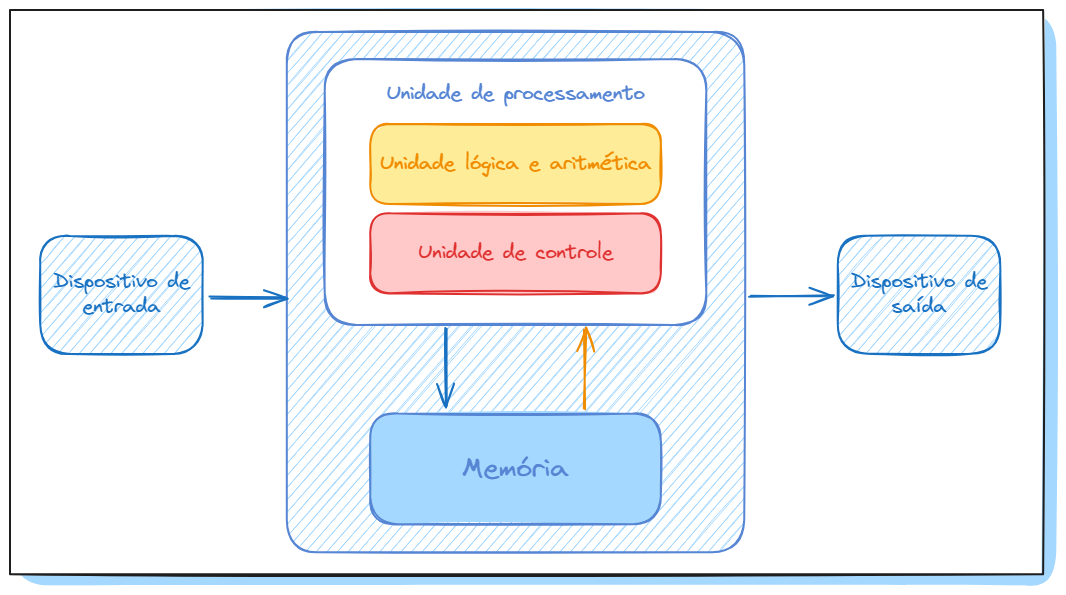
\includegraphics[scale=0.30]{../assets/img/von-neumann.png}
	\legend{Fonte: Autoria própria}
\end{figure}

Nesse tipo de arquitetura, o processador pode ler apenas uma instrução OU dado
por vez. Isso porque ambas as leituras ocorrem por meio do mesmo barramento.

A arquitetura apresentada na seção \ref{sec:6502} segue exatamente os mesmos
princípios apresentados aqui: um único barramento de endereços no qual o
processador pode comunicar qual o endereço da informação que está tentando
acessar, e um barramento de dados por onde a informação se propaga.

É importante também destacar que ainda que seja possível fisicamente separar
as memórias de dados e de programa (o que de fato é algo que será feito) durante
esse trabalho, do ponto de vista do processador essa não é uma diferença efetiva.
O processador apenas consegue ``enxergar'' um único barramento de dados e de
endereço, não importa quais dispositivos estejam conectados diretamente.

\section{Microprocessador 6502} \label{sec:6502}
O microprocessador 6502 é o segundo membro da família MCS650X. Essa família de
microprocessadores de 8 bits foi lançada em 1975 pela \emph{MOS Technology}.
Os processadores dessa família apresentam o mesmo conjunto de instruções e modos
de endereçamento, com pequenas diferenças em recursos e sua utilização
\cite{mosHardware1976}. Por conta de sua eficácia e baixo custo, o
microprocessador se popularizou rapidamente ao ser usado em diversos sistemas
da época como \emph{O Nintendo Entertainment System (NES)}, \emph{Apple II},
\emph{Commodore 64} e muitos outros.
\subsection{Arquitetura Original}
O microprocessador conta com um Barramento de Dados de 8 bits e um Barramento de
endereços 16-bits. Qualquer operação que o processador precisa executar
normalmente é iniciada colocando o endereço de acesso no Barramento de endereços
e posteriormente lendo (ou escrevendo) um valor de 8-bits no Barramento de dados.

Internamente, 3 registradores de propósito geral podem ser usados.
\begin{itemize}
	\item \textbf{Acumulador (A)}: Usado também para armazenar o resultado das
	      operações lógicas e aritméticas;
	\item \textbf{\emph{Index} X e Y}: Ambos os registradores podem ser usados
	      para operações com modos de endereçamento especiais, que serão abordados
	      mais a frente no relatório.
\end{itemize}

Além dos 3 registradores que podem ser acessados diretamente, o 6502 também
possuí alguns registradores usados por funções específicas do processador.

\subsection{Registrador de Status (SR)} \label{statusReg}

O \textbf{registrador de status} é responsável por armazenar \emph{flags} usadas
para o controle do fluxo de programa do processador. Elas normalmente são
atualizadas durante operações lógicas, aritméticas e de transferência de dados.
\begin{itemize}
	\item \textbf{\emph{Carry (C)}}: Indica se a operação gerou um \emph{carry};
	\item \textbf{Negativo (N)}: Indica se a operação gerou um valor com o bit
	      mais significativo ativo;
	\item \textbf{\emph{Overflow} (V)}: Indica se a operação gerou um...;
	\item \textbf{Zero (Z)}: Indica se a operação gerou o valor zero;
	\item \textbf{Decimal (D)}: Indica se o processador está em modo aritmético
	      decimal BCD;
	\item \textbf{Bloqueio de interrupções (I)}: Indica se o processador está
	      ignorando as requisição de interrupções;
	\item \textbf{\emph{Break} (B)}: Indica se a interrupção atual foi disparada
	      via \emph{software} pela instrução BRK, ao invés de uma interrupção via
	      \emph{hardware}.
\end{itemize}

\subsection{Contador de Programa (PC)}
O único registrador de 16-bits definido pela arquitetura. Esse registrador é
responsável por manter o endereço de memória atualmente acessado pelo
processador.

\subsection{\emph{Stack Pointer} (SP)}
O \emph{stack} é uma região de memória destinada para rápido acesso e escrita.
A eficácia nessas operações vem do fato de que o processador utiliza o endereço
no SP para saber exatamente onde a próxima leitura e escrita vai ocorrer.
O registrador é incrementado ou decrementado de acordo após cada operação. O
6502 também utiliza o \emph{stack} para armazenar os endereços de retorno quando
subrotinas ou interrupções são executadas.

\subsection{Modos de endereçamento}
O 6502 é capaz de endereçar 65.536 bytes de memória. Qualquer operação ou
estrutura de dados dentro do processador compartilham esse mesmo espaço de
memória. O processador também providencia 13 diferentes métodos de calcular o
endereço efetivo de memória na qual a operação vai ser executada
\cite{w65c02sDatasheet}. Na computação, chamamos esses métodos de
\textbf{modos de endereçamento} e aqueles disponíveis no 6502 serão descritos
aqui.

\subsubsection{Endereçamento imediato}
Nesse tipo de instrução o operando é usado imediatamente após a instrução ter
sido lida. Nenhum acesso a memória ou cálculo é realizado
(\autoref{fig:address:imm}). Essa tipo de instrução utiliza 2 bytes de memória.

\begin{figure}[h]
	\centering
	\caption{Endereçamento imediato} \label{fig:address:imm}
	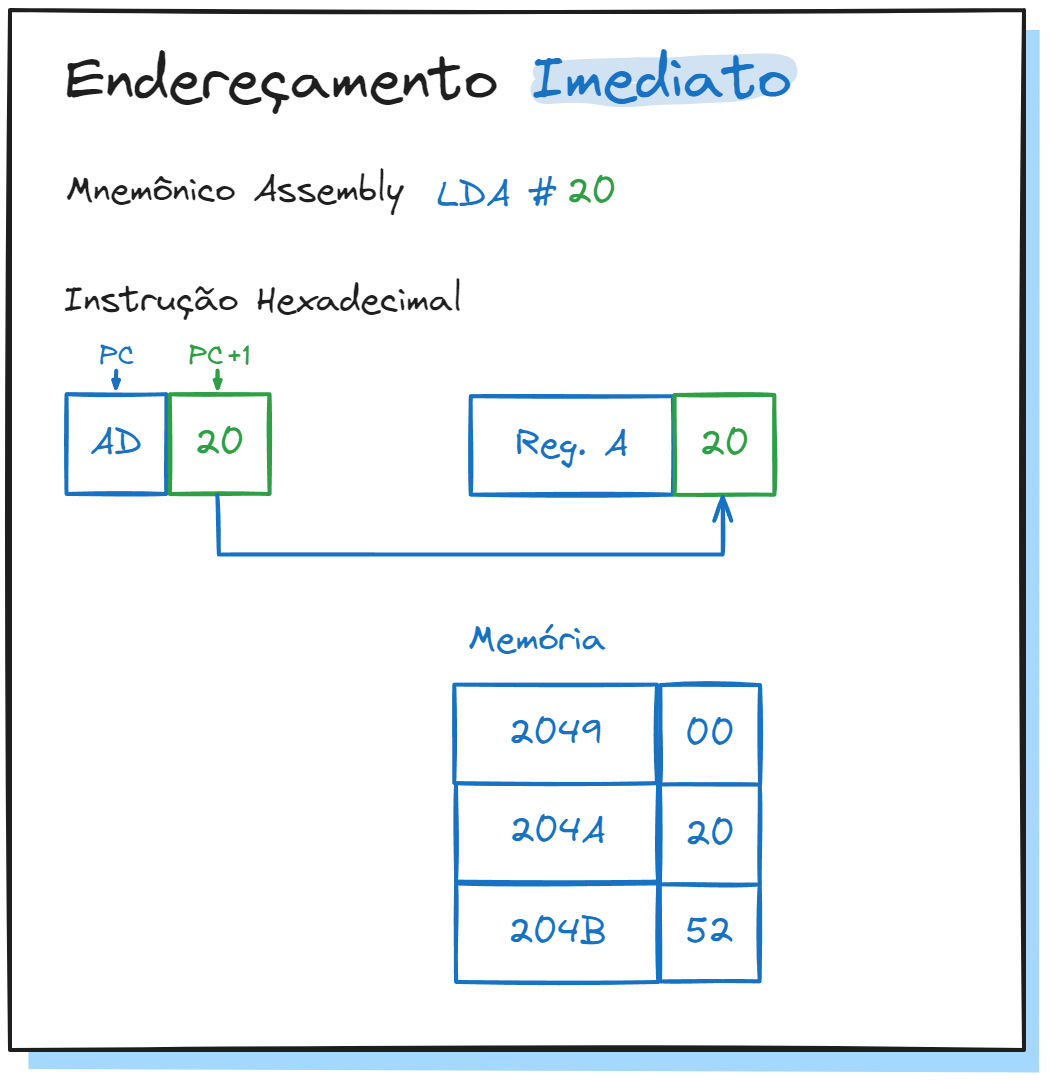
\includegraphics[scale=0.25]{../assets/img/addressing-modes-imm.png}
	\legend{Fonte: Autoria própria}
\end{figure}

\subsubsection{Endereçamento absoluto}
Nesse tipo de instrução dois bytes são passados além do opcode. O processador
usa esses bytes como um endereço de acesso a memória (\autoref{fig:address:abs}).
\begin{figure}[h]
	\centering
	\caption{Endereçamento absoluto. Note que o primeiro byte na memória é o menos
		significativo}
	\label{fig:address:abs}
	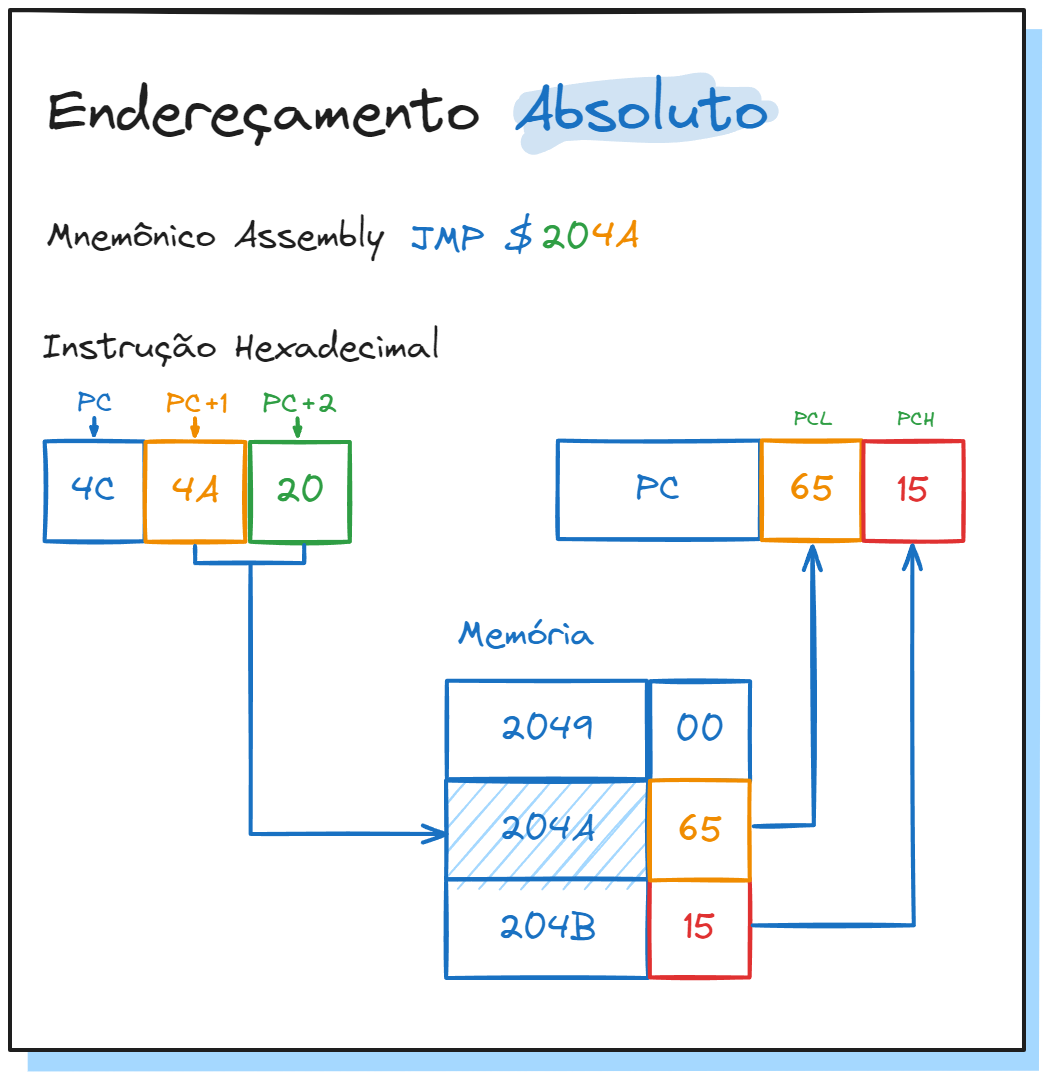
\includegraphics[scale=0.25]{../assets/img/addressing-modes-abs.png}
	\legend{Fonte: Autoria própria}
\end{figure}

\subsubsection{Endereçamento absoluto - Deslocado em X (ou Y)}
Esse modo é uma variação do endereçamento absoluto: dois bytes são buscados da
memória e usados como endereço de acesso. A diferença está no fato de que o
valor do registrador (X ou Y) é somado ao endereço de acesso.
(\autoref{fig:address:absx}).
\begin{figure}[h]
	\centering
	\caption{Endereçamento absoluto - Deslocado em X (ou Y)}
	\label{fig:address:absx}
	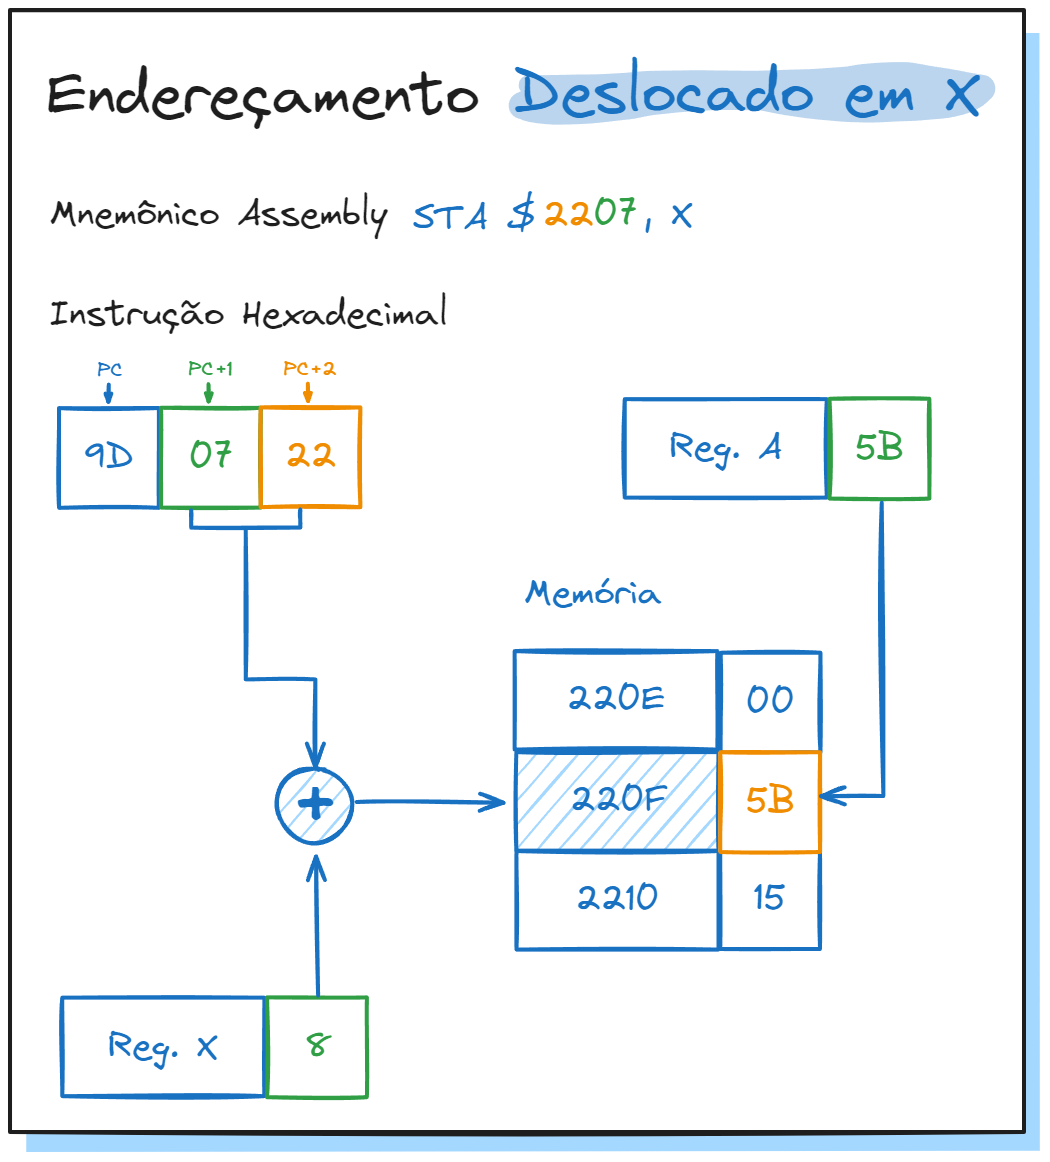
\includegraphics[scale=0.25]{../assets/img/addressing-modes-absx.png}
	\legend{Fonte: Autoria própria}
\end{figure}

\subsubsection{Endereçamento \emph{Zero-Page}}
Idêntico ao endereçamento absoluto, exceto que apenas um byte é lido da memória
(o byte menos significativo). O byte mais significativo é inferido como 0
\autoref{fig:address:zpg}. Logo esse modo de endereçamento sempre retorna um
dado localizado na primeira ``página'' da memória (os primeiros 256 bytes).
\begin{figure}[h]
	\centering
	\caption{Endereçamento \emph{Zero-Page}} \label{fig:address:zpg}
	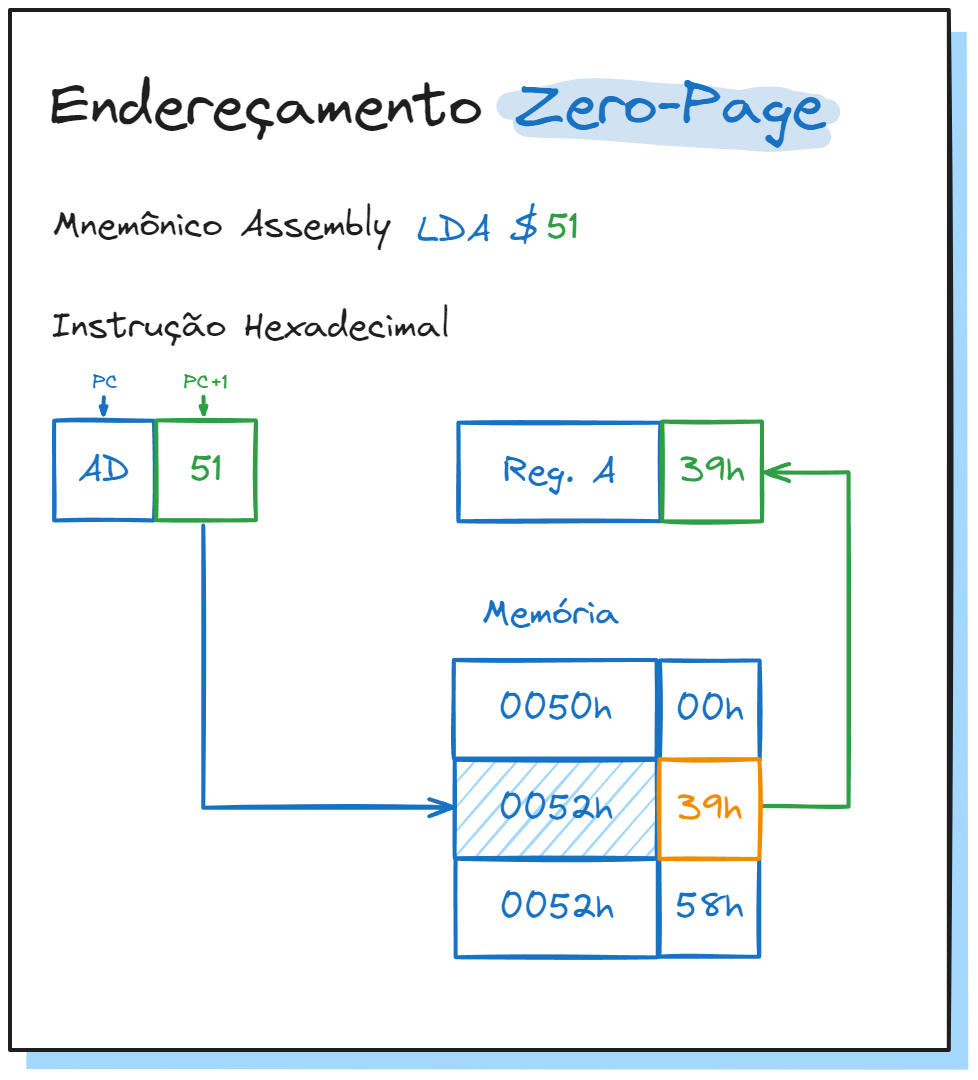
\includegraphics[scale=0.25]{../assets/img/addressing-modes-zpg.png}
	\legend{Fonte: Autoria própria}
\end{figure}

\subsubsection{Endereçamento relativo}
O endereçamento relativo é usado especificamente para instruções de
\emph{branch}. Nele, o operando contém um valor que será somado ao valor atual
do Contador de Programa. Esse valor é então colocado de volta no Contador de
programa para que a execução possa continuar a partir daí.
É importante destacar que o byte de deslocamento passado nessa instrução pode
possuir sinal positivo ou negativo. Isso significa pular para um endereço
posterior ou anterior contando que o valor de deslocamento esteja entre -128
e 127.
\begin{figure}[h]
	\centering
	\caption{Endereçamento relativo} \label{fig:address:rel}
	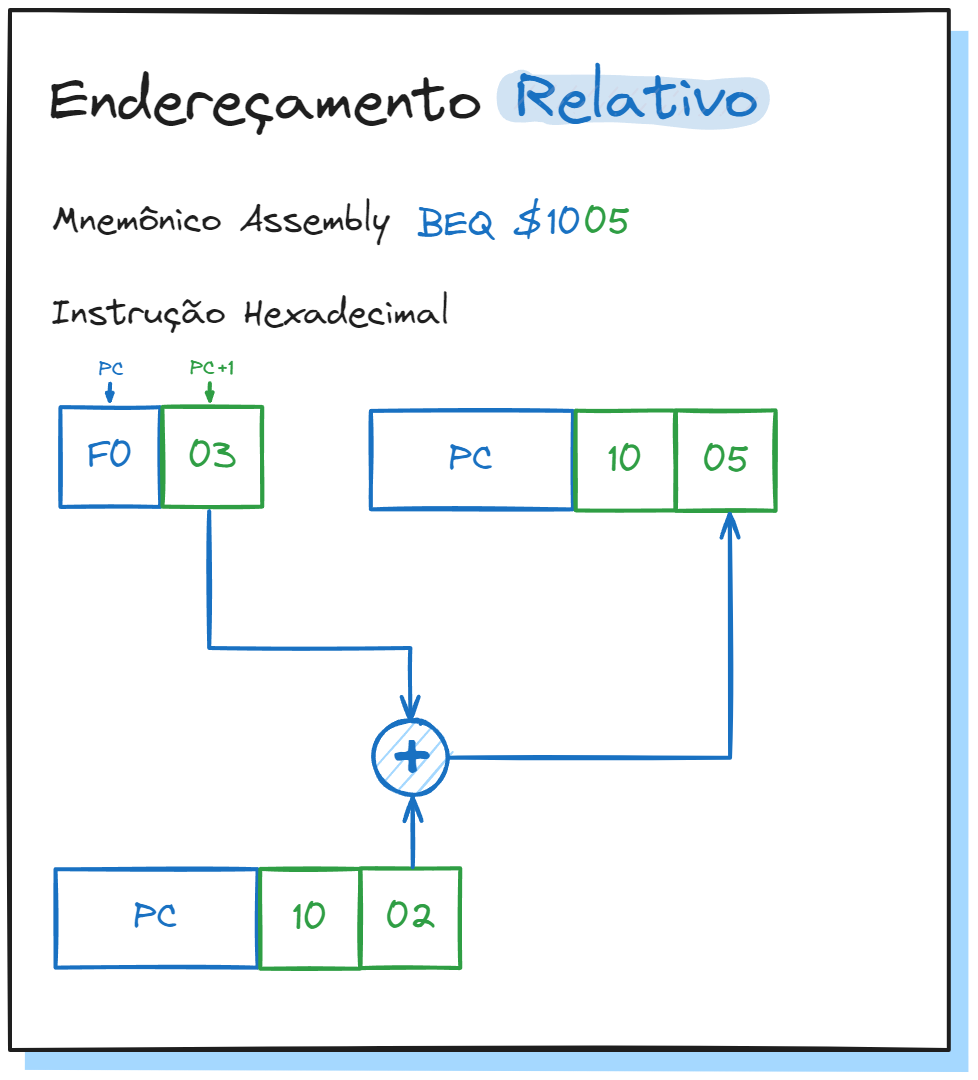
\includegraphics[scale=0.25]{../assets/img/addressing-modes-rel.png}
	\legend{Fonte: Autoria própria}
\end{figure}

\subsubsection{Endereçamento indireto}
Nesse tipo de endereçamento, o processador busca o endereço efetivo no endereço
que foi passado pelo operando (\autoref{fig:address:ind}).
\begin{figure}[h]
	\centering
	\caption{Endereçamento indireto} \label{fig:address:ind}
	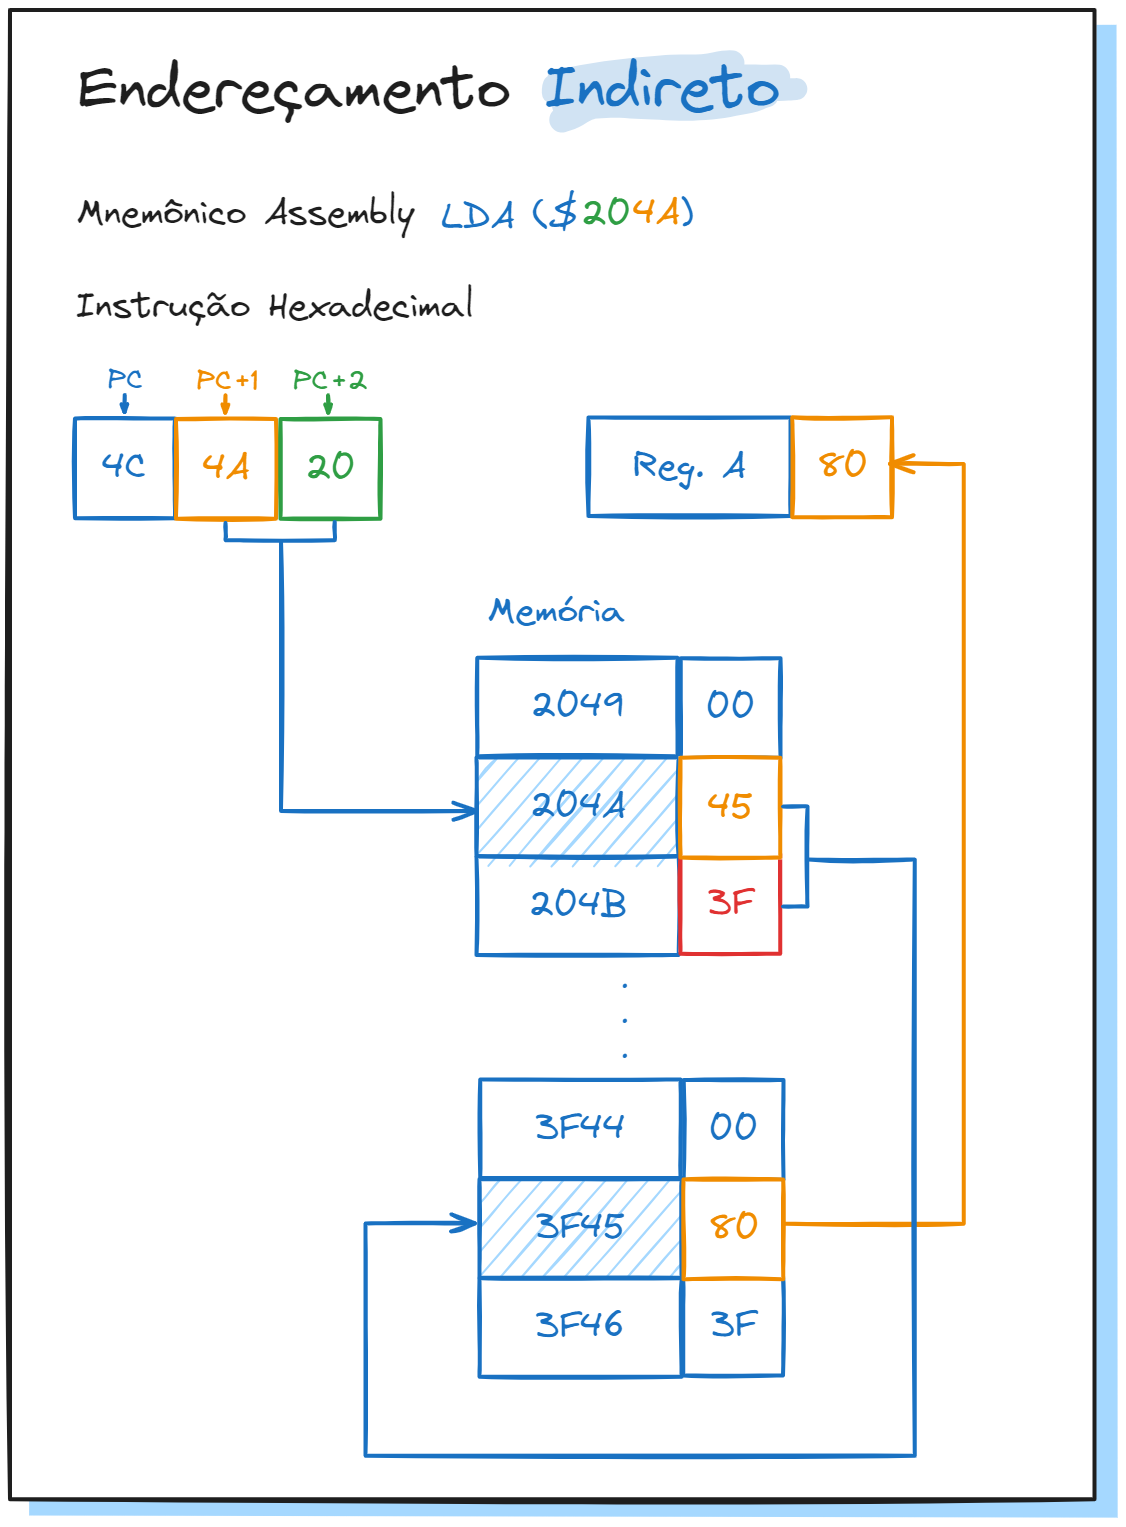
\includegraphics[scale=0.25]{../assets/img/addressing-modes-ind.png}
	\legend{Fonte: Autoria própria}
\end{figure}

\subsection{Endereçamento \emph{Zero-Page}, deslocado em X (ou Y)}
Idêntico ao Endereçamento Absoluto deslocado em X (ou Y), exceto que o endereço
de acesso está sempre nos primeiros 256 bytes do espaço de memória
(\autoref{fig:address:absx}).

\section{RTL - \emph{Register-Transfer Logic}}
Quando tratamos do design de circuitos digitais complexos, é comum abstrairmos
diferentes níveis do design com a intenção de tornar esses problemas mais
simples de serem resolvidos.

3 níveis diferentes de abstração são definidos por \citeonline{vahid2011} na
construção de circuitos digitais:
\begin{enumerate}
	\item \textbf{\emph{Transistor Level}}: Conectar transistores para construir
	      componentes lógicos.
	\item \textbf{\emph{Logic Level}}: Utilizar-se de Portas Lógicas como bloco
	      principal de construção para desenvolver circuitos combinacionais.
	\item \textbf{\emph{Register-transfer Level}}: Conectar uma rede de
	      registradores e construir blocos que definem a lógica de transferência
	      de estado entre esses registradores.
\end{enumerate}

De maneira geral, no \emph{Register-Transfer Level Design} (ou Design RTL) cada
bloco do design deve desempenhar uma (e apenas uma) de duas possíveis funções:
\begin{enumerate}
	\item \textbf{Lógica Combinacional}: São os blocos responsáveis pela
	      computação do próximo estado. De maneira geral, esses blocos devem ser
	      determinísticos e sempre apresentar a mesma saída para uma determinada
	      entrada.
	\item \textbf{Lógica Sequencial}: São blocos responsáveis por guardar e
	      propagar o estado computado pelos blocos combinacionais de maneira
	      síncrona.
\end{enumerate}

\begin{table}[htb]
	\centering
	\ABNTEXfontereduzida
	\caption{Tamanho da instrução por modo de endereçamento} \label{tab:Instr3OP}
	\begin{tabular}{|l|c|}
		\hline
		\textbf{Modo de endereçamento}            & \textbf{Tamanho em bytes} \\ \hline
		Acumulador (A)                            & 1                         \\ \hline
		Absoluto (abs)                            & 3                         \\ \hline
		Absoluto, deslocado em X (abs, x)         & 3                         \\ \hline
		Absoluto, deslocado em Y (abs, y)         & 3                         \\ \hline
		Imediato (\#)                             & 2                         \\ \hline
		Implícito (impl)                          & 1                         \\ \hline
		Indireto (ind)                            & 3                         \\ \hline
		Indireto, deslocado em X (X, ind)         & 2                         \\ \hline
		Indireto, deslocado em Y (ind, Y)         & 2                         \\ \hline
		Relativo (rel)                            & 2                         \\ \hline
		\emph{Zero-Page} (zpg)                    & 2                         \\ \hline
		\emph{Zero-Page}, deslocado em X (zpg, x) & 2                         \\ \hline
		\emph{Zero-Page}, deslocado em Y (zpg, y) & 2                         \\ \hline
	\end{tabular}
	\legend{Fonte: Autoria Própria}
\end{table}


% \section{FPGA - Field Programmable Array}

% \section{Verilog Sintetizável}

% \section{Completude de Turing}

\section{Metodologia de Testes}

Para garantir o funcionamento das partes individuais do processador, a ferramenta
de simulação digital ModelSim da Intel foi utilizada.

Um template para os testbenches está disponível no \autoref{attach:template}

\chapter{Desenvolvimento}

O desenvolvimento da CPU se deu em algumas etapas. Primeiramente o conjunto de
instrução foi definido como um subconjunto da família MCS650X original. Depois
disso foram escolhidos alguns modos de endereçamento e um \emph{datapath} foi
definido.

\section{Conjunto de instruções}
O conjunto de instruções apresentado na \autoref{tab:instSet} é apenas um
subconjunto da família MCS650X original. Os mesmos \emph{opcodes} da arquitetura
original serão mantidos aqui \cite{6502isa}.

\begin{center}
	\fontsize{9}{11}\selectfont
	\begin{longtable}{|l|c|c|c|p{7cm}|}
		\caption{Conjunto de instruções} \label{tab:instSet}                                                                                   \\
		\hline
		\multicolumn{5}{|c|}{\textbf{Instruções de transferência}}                                                                             \\ \hline
		\textbf{Instrução}   & \textbf{Opcode} & \textbf{Mod. End} & \textbf{Assembly}      & \textbf{Operação}                                \\ \hline
		\multirow{3}{*}{LDA} & a9              & imm               & \codenobg{LDA imm}     & \codenobg{RegAC <= imm}                          \\ \cline{2-5}
		                     & ad              & abs               & \codenobg{LDA addr}    & \codenobg{RegAC <= Mem[addr]}                    \\ \cline{2-5}
		                     & bd              & (abs, x)          & \codenobg{LDA addr, x} & \codenobg{RegAC <= Mem[addr + x]}                \\ \hline
		\multirow{3}{*}{LDX} & a2              & imm               & \codenobg{LDX imm}     & \codenobg{RegX <= imm}                           \\ \cline{2-5}
		                     & ae              & abs               & \codenobg{LDX addr}    & \codenobg{RegX <= Mem[addr]}                     \\ \cline{2-5}
		                     & be              & (abs, y)          & \codenobg{LDY addr, y} & \codenobg{RegY <= Mem[addr + x]}                 \\ \hline
		\multirow{3}{*}{LDY} & a0              & imm               & \codenobg{LDY imm}     & \codenobg{RegY <= imm}                           \\ \cline{2-5}
		                     & ac              & abs               & \codenobg{LDY addr}    & \codenobg{RegY <= Mem[addr]}                     \\ \cline{2-5}
		                     & bc              & (abs, x)          & \codenobg{LDY addr, x} & \codenobg{RegY <= Mem[addr + x]}                 \\ \hline
		\multirow{2}{*}{STA} & 8d              & abs               & \codenobg{STA addr}    & \codenobg{Mem[addr]<= RegAC}                     \\ \cline{2-5}
		                     & 9d              & (abs, x)          & \codenobg{STA addr, x} & \codenobg{Mem[addr + x]<= RegAC}                 \\ \hline
		\multirow{1}{*}{STX} & 8e              & abs               & \codenobg{STX addr}    & \codenobg{Mem[addr]<= RegX}                      \\ \hline
		\multirow{1}{*}{STY} & 8c              & abs               & \codenobg{STY addr}    & \codenobg{Mem[addr]<= RegY}                      \\ \hline
		\multicolumn{5}{|c|}{\textbf{Instruções lógicas e aritméticas}}                                                                        \\ \hline
		\textbf{Instrução}   & \textbf{Opcode} & \textbf{Mod. End} & \textbf{Assembly}      & \textbf{Operação}                                \\ \hline
		\multirow{3}{*}{ADC} & 69              & imm               & \codenobg{ADC imm}     & \codenobg{RegAC <= RegAC + imm + C}              \\ \cline{2-5}
		                     & 6d              & abs               & \codenobg{ADC addr}    & \codenobg{RegAC <= RegAC + Mem[addr] + C}        \\ \cline{2-5}
		                     & 7d              & (abs, x)          & \codenobg{ADC addr, x} & \codenobg{RegAC <= RegAC + Mem[addr + x] + C}    \\ \hline
		\multirow{3}{*}{SBC} & e9              & imm               & \codenobg{SBC imm}     & \codenobg{RegAC <= RegAC - imm - C}              \\ \cline{2-5}
		                     & ed              & abs               & \codenobg{SBC addr}    & \codenobg{RegAC <= RegAC - Mem[addr] - C}        \\ \cline{2-5}
		                     & fd              & (abs, x)          & \codenobg{SBC addr, x} & \codenobg{RegAC <= RegAC - Mem[addr + x] - C}    \\ \hline
		\multirow{3}{*}{AND} & 29              & imm               & \codenobg{AND imm}     & \codenobg{RegAC <= RegAC AND imm}                \\ \cline{2-5}
		                     & 2d              & abs               & \codenobg{AND addr}    & \codenobg{RegAC <= RegAC AND Mem[addr]}          \\ \cline{2-5}
		                     & 3d              & (abs, x)          & \codenobg{AND addr, x} & \codenobg{RegAC <= RegAC AND Mem[addr + x]}      \\ \hline
		\multirow{3}{*}{EOR} & 49              & imm               & \codenobg{EOR imm}     & \codenobg{RegAC <= RegAC XOR imm}                \\ \cline{2-5}
		                     & 4d              & abs               & \codenobg{EOR addr}    & \codenobg{RegAC <= RegAC XOR Mem[addr]}          \\ \cline{2-5}
		                     & 5d              & (abs, x)          & \codenobg{EOR addr, x} & \codenobg{RegAC <= RegAC XOR Mem[addr + x]}      \\ \hline
		\multirow{2}{*}{ORA} & 09              & imm               & \codenobg{ORA imm}     & \codenobg{RegAC <= RegAC OR imm}                 \\ \cline{2-5}
		                     & 0d              & abs               & \codenobg{ORA addr}    & \codenobg{RegAC <= RegAC OR Mem[addr]}           \\ \hline
		\multirow{1}{*}{ORA} & 1d              & (abs, x)          & \codenobg{ORA addr, x} & \codenobg{RegAC <= RegAC OR Mem[addr + x]}       \\ \hline
		\multicolumn{5}{|c|}{\textbf{Comparação}}                                                                                              \\ \hline
		\textbf{Instrução}   & \textbf{Opcode} & \textbf{Mod. End} & \textbf{Assembly}      & \textbf{Operação}                                \\ \hline
		\multirow{3}{*}{CMP} & c9              & imm               & \codenobg{CMP imm}     & \codenobg{C, N, V, Z <= ACC - imm }              \\ \cline{2-5}
		                     & cd              & abs               & \codenobg{CMP addr}    & \codenobg{C, N, V, Z <= ACC - Mem[addr] }        \\ \cline{2-5}
		                     & dd              & (abs, x)          & \codenobg{CMP addr, x} & \codenobg{C, N, V, Z <= ACC - Mem[addr - x] }    \\ \hline
		\multicolumn{5}{|c|}{\textbf{Flags}}                                                                                                   \\ \hline
		\textbf{Instrução}   & \textbf{Opcode} & \textbf{Mod. End} & \textbf{Assembly}      & \textbf{Operação}                                \\ \hline
		\multirow{1}{*}{SEC} & 38              & impl              & \codenobg{SEC}         & \codenobg{C <= 1}                                \\ \hline
		\multirow{1}{*}{CLC} & 18              & impl              & \codenobg{CLC}         & \codenobg{C <= 0}                                \\ \hline
		\multicolumn{5}{|c|}{\textbf{Instruções de \emph{branch}}}                                                                             \\ \hline
		\textbf{Instrução}   & \textbf{Opcode} & \textbf{Mod. End} & \textbf{Assembly}      & \textbf{Operação}                                \\ \hline
		\multirow{1}{*}{BCC} & 90              & rel               & \codenobg{BCC}         & \codenobg{branch on C = 0}                       \\ \hline
		\multirow{1}{*}{BCS} & b0              & rel               & \codenobg{BCS}         & \codenobg{branch on C = 1}                       \\ \hline
		\multirow{1}{*}{BEQ} & f0              & rel               & \codenobg{BEQ}         & \codenobg{branch on Z = 1}                       \\ \hline
		\multirow{1}{*}{BMI} & 30              & rel               & \codenobg{BMI}         & \codenobg{branch on N = 1}                       \\ \hline
		\multirow{1}{*}{BNE} & d0              & rel               & \codenobg{BNE}         & \codenobg{branch on Z = 0}                       \\ \hline
		\multirow{1}{*}{BPL} & 10              & rel               & \codenobg{BPL}         & \codenobg{branch on N = 0}                       \\ \hline
		\multirow{1}{*}{BVC} & 50              & rel               & \codenobg{BVC}         & \codenobg{branch on V = 0}                       \\ \hline
		\multirow{1}{*}{BVS} & 70              & rel               & \codenobg{BVS}         & \codenobg{branch on V = 1}                       \\ \hline
		\multicolumn{5}{|c|}{\textbf{Instruções de controle}}                                                                                  \\ \hline
		\multirow{1}{*}{JMP} & 6c              & abs               & \codenobg{JMP HHLL}    & \codenobg{PCL <= LL}\newline\codenobg{PCH <= HH} \\ \hline
		\multirow{1}{*}{NOP} & ea              & impl              & \codenobg{NOP}         &                                                  \\ \hline
		\multirow{1}{*}{HLT} & db              & impl              & \codenobg{HLT}         &                                                  \\ \hline
	\end{longtable}
	\legend{Fonte: Autoria Própria}
\end{center}


\section{O \emph{datapath} da implementação}
A \autoref{fig:6502} mostra o \emph{datapath} que será implementado durante esse
trabalho.

O processador possuí 3 registradores de propósito geral e é capaz de manipular
8-bits por ciclo de clock, por consequência toda instrução no 6502 leva mais de
1 ciclo para ser executada, considerando que o opcode consiste sempre de 8-bits.

A \autoref{fig:6502} também divide os componentes em dois grupos principais:
\begin{itemize}
	\item \textbf{Registradores externos}: São os registradores que o programador
	      tem consciência que estão lá e pode, por meio do conjunto de instruções,
	      interagir com eles de maneira direta ou indireta.
	\item \textbf{Microarquitetura interna}: São os componentes internos que não
	      são diretamente definidos pela arquitetura MCS650X, são invisíveis do
	      ponto de vista do programador mas são vitais para o funcionamento do
	      processador.
\end{itemize}

O processador possuí uma Barramento de Endereços de 16-bits, isso significa que
ele se comunicar com até 65,536 diferente endereços. Esse diferentes endereços
serão mencionados daqui em diante como o Espaço de Memória (EM) do 6502.

\section{Unidades funcionais}
Essa seção apresenta uma breve descrição de cada componente no \emph{datapath}.

\subsection{Registradores de propósito geral (AC, X, Y)}
Esses registradores de 8-bits que podem ser acessados diretamente utilizando
suas respectivas instruções de \emph{Load} e \emph{Store}. Além disso, eles
desempenham funções específicas no processador:
\begin{itemize}
	\item \textbf{Acumulador (AC)}: Toda operação lógica e aritmética tem como
	      base o valor armazenado nesse registrador, além disso o resultado dessas
	      operações também é diretamente armazenado aqui.
	\item \textbf{X e Y}: Esses registradores armazenam o valor de deslocamento
	      das instruções com os modos de endereçamento deslocados.
\end{itemize}


\begin{figure}[h]
	\centering
	\caption{Datapath do 6502 implementado} \label{fig:6502}
	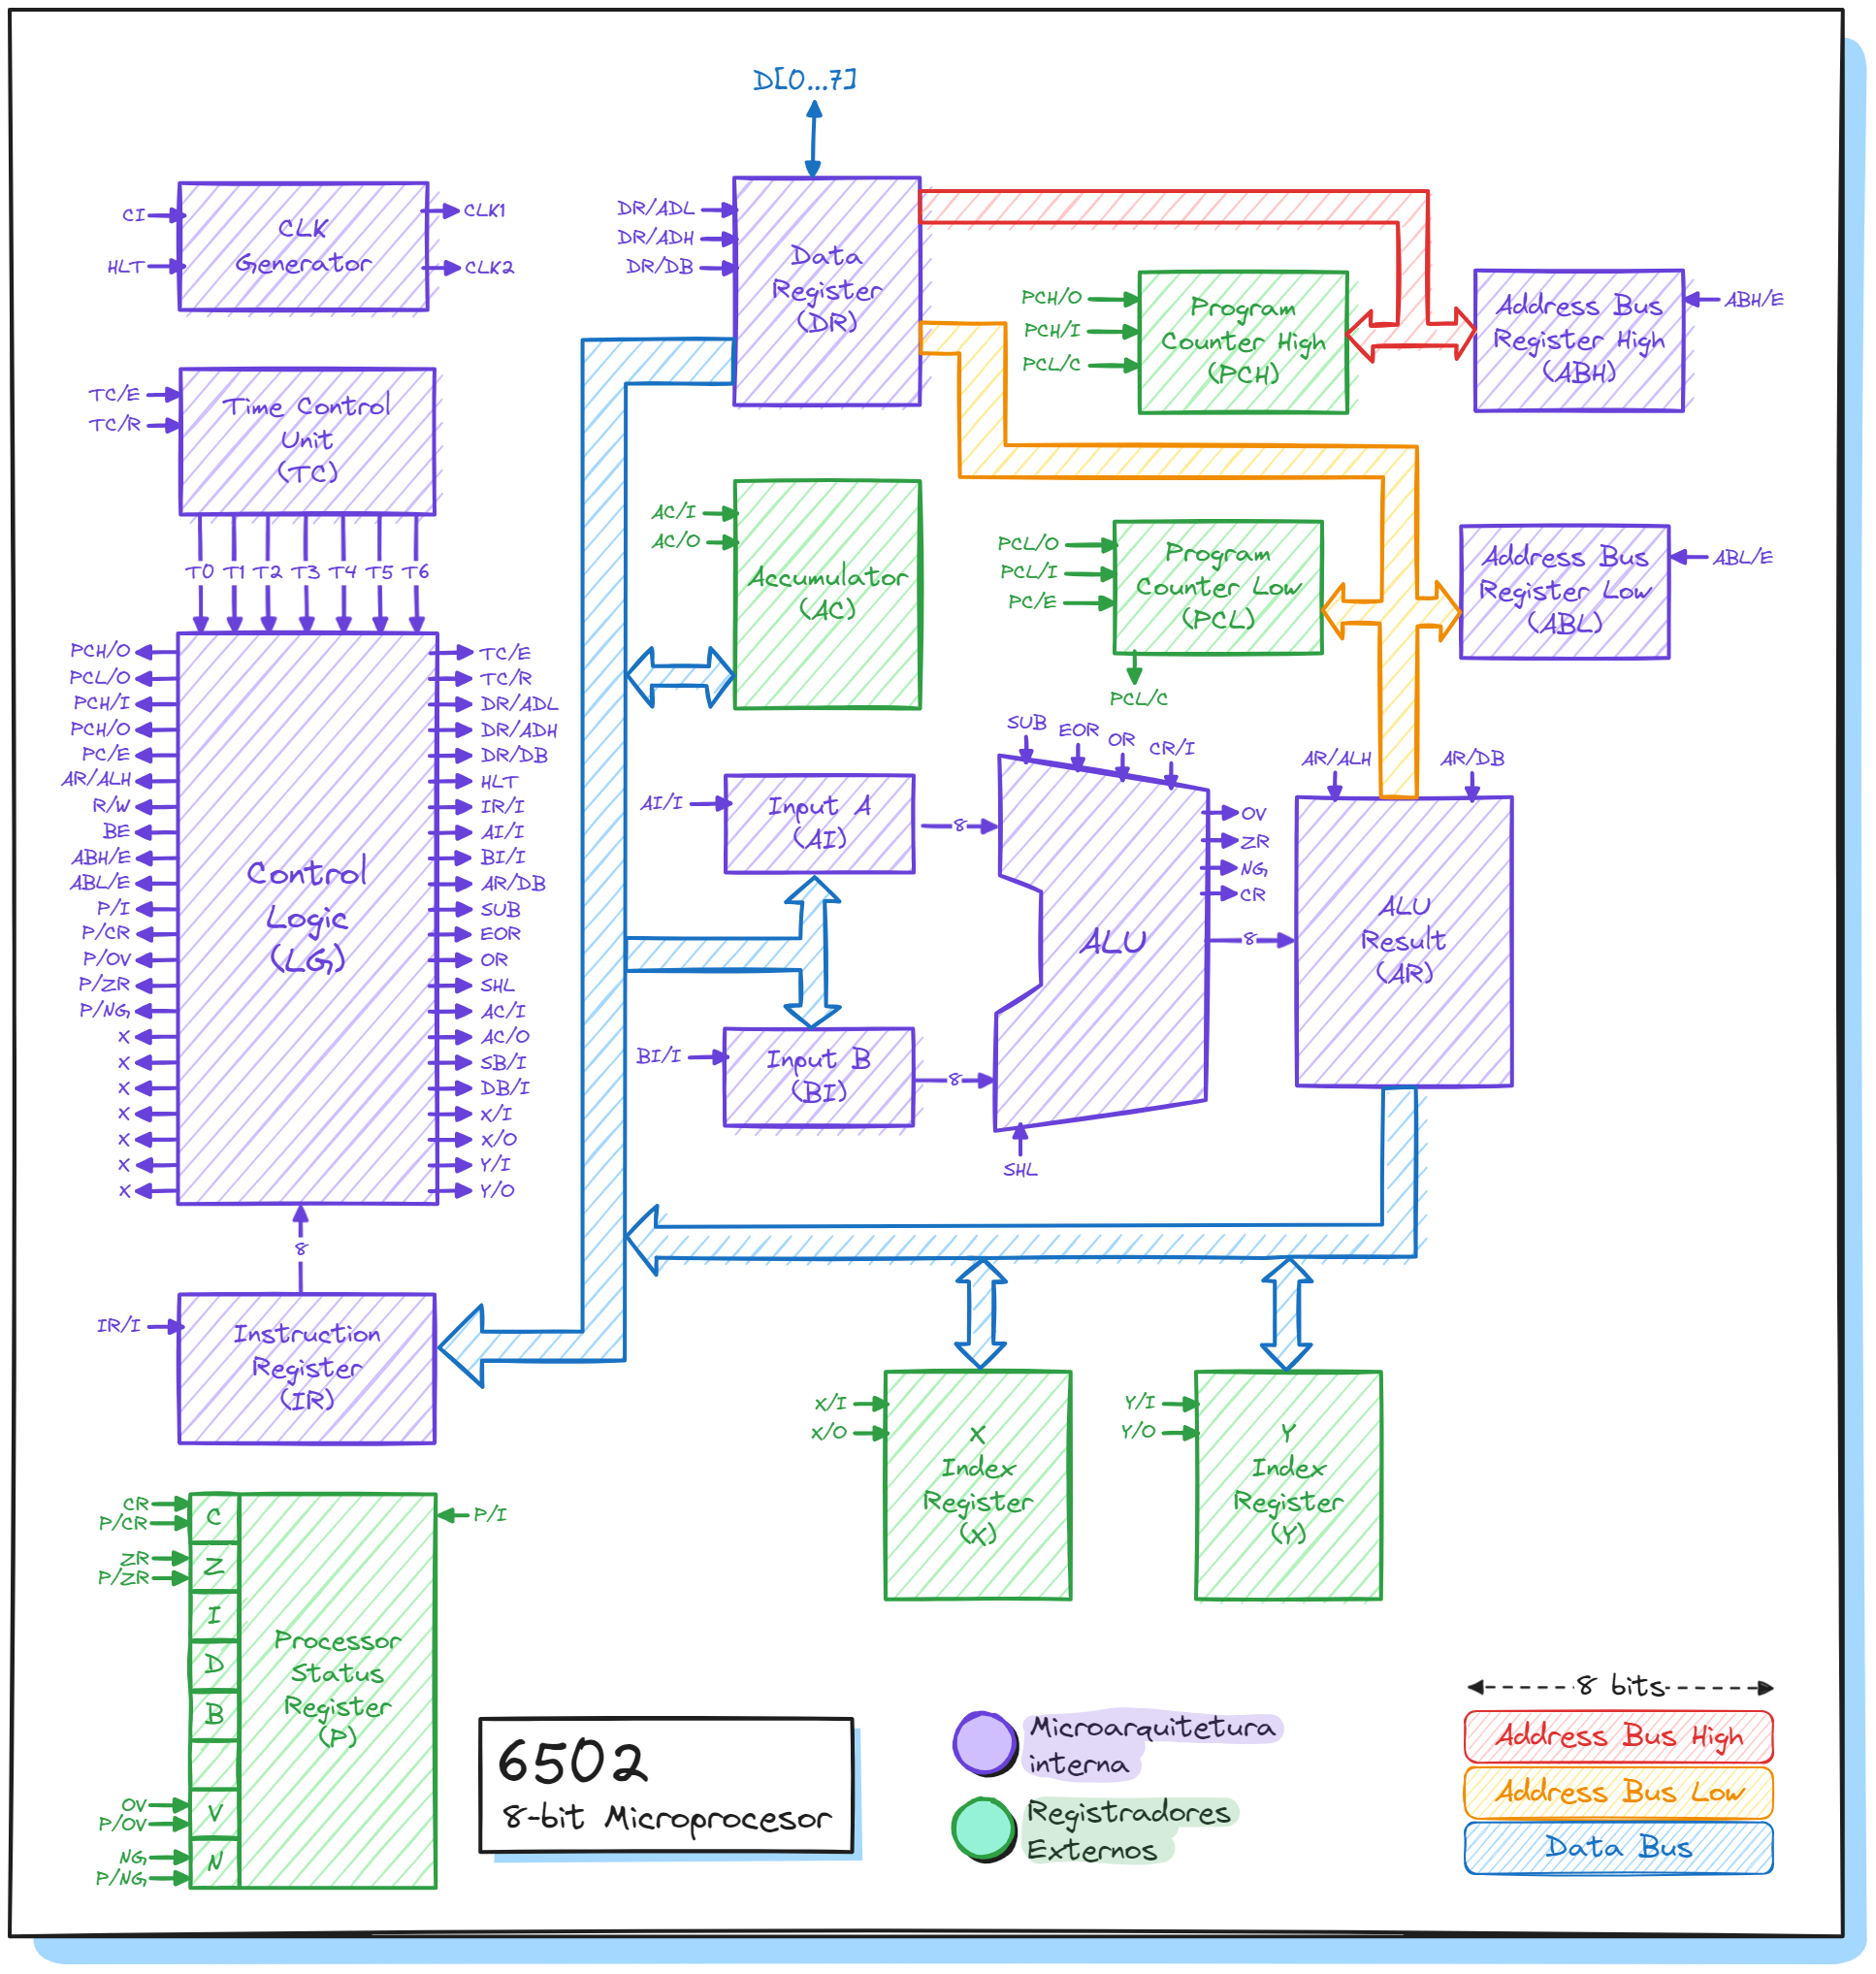
\includegraphics[scale=0.22]{../assets/img/6502.png}
\end{figure}

\subsection{Contador de Programa (PCH e PCL)}

O contador de programa é usado para endereçar o espaço de 16-bits de memória
disponível para o processador. Por conta do processador conseguir manipular
apenas 8-bits por vez, utiliza-se 2 registradores de 8 bits para armazenar o
endereço completo. O programador pode manipular seu valor por meio das
instruções de \emph{jump} e \emph{branch}.

\subsection{Registrador de Dados (DR)}
O registrador de dados é responsável por controlar a entrada de informações
no processador e distribuir para um dos 3 barramentos disponíveis.

\subsection{Registrador de Status (P)}
Essa implementação difere da apresentada em \ref{statusReg}. As \emph{flags} I,
D e B não serão implementadas.
Os outros valores serão controlados pelo resultado de operações aritméticas,
\emph{loads} e \emph{stores}.

\subsection{Unidade de controle}
A unidade de controle é responsável por enviar todos os sinais de controle
necessários para a execução de uma instrução em particular. Ela é composta por 3
partes:
\begin{enumerate}
	\item \textbf{Registrador de instrução (IR)}: Armazena o \emph{opcode} da
	      instrução atualmente sendo executada.
	\item \textbf{Unidade de tempo (TCU)}: No começo de toda instrução, seu valor
	      é definido como T0, na \textbf{descida} de cada ciclo de clock seu valor é
	      incrementado (T1, T2, T3, etc).
	\item \textbf{Lógica de Controle (LG)}: Responsável por definir todos os
	      sinais de controle baseado na instrução que está sendo executado atualmente
	      (armazenada no IR) e qual ciclo o processador se encontra dentro dessa
	      instrução (armazenado no TCU).
\end{enumerate}

\subsection{Geração de \emph{Clock} (CLK)}
Essa unidade é responsável por gerar o sinal de clock do processador. O clock de
entrada (CI) é dividido em 2 clocks espelhados. Diferentes componentes podem
executar operações em um dos dois ciclos de \emph{clocks}.

\subsection{Registrador do barramento de endereço (ABL e ABH)}
O endereço que está sendo acessado atualmente pelo processador ficará armazenado
nesse registrador. Como o endereço é de 16-bits, 2 registradores de 8-bits serão
usados.

\subsection{Unidade Lógica aritmética (ALU)}
A ALU é o circuito combinacional responsável por executar todas as operações
lógicas e aritméticas do processador. Além disso, registradores auxiliares são
acoplados a unidade: AI e BI armazenam os valores de entrada e AR armazena o
valor de saída.

\section{Código Fonte do Processador}

O código do processador é apresentado nessa seção. Os componentes de \emph{datapath}
são descritos em \nameref{code:alu}, \nameref{code:program_counter},
\nameref{code:register} e \nameref{code:status_register}. O \nameref{code:register}
é usado para implementar os registradores de propósito geral Acumulador, X e Y.

\nameref{code:bus_sources}, \nameref{code:control_signals} e \nameref{code:instruction_set} são usados
para providenciar constantes que são usadas pelos diversos módulos do projeto.

\begin{longlisting}
	\caption[Enums para barramentos]{bus{\_}sources.sv}
	\inputminted{systemverilog}{../quartus/synthesis/enums/bus_sources.sv}
	\label{code:bus_sources}
\end{longlisting}

\begin{longlisting}
	\caption[Enums para sinais de controle]{control{\_}signals.sv}
	\inputminted{systemverilog}{../quartus/synthesis/enums/control_signals.sv}
	\label{code:control_signals}
\end{longlisting}

\begin{longlisting}
	\caption[Enums para conjunto de instrução]{instruction{\_}set.sv}
	\inputminted{systemverilog}{../quartus/synthesis/enums/instruction_set.sv}
	\label{code:instruction_set}
\end{longlisting}

\begin{longlisting}
	\caption[Módulo ULA]{alu.sv}
	\inputminted[firstline=5]{systemverilog}{../quartus/synthesis/alu.sv}
	\label{code:alu}
\end{longlisting}


\begin{longlisting}
	\caption[Módulo Contador de Programa]{program{\_}counter.sv}
	\inputminted{systemverilog}{../quartus/synthesis/program_counter.sv}
	\label{code:program_counter}
\end{longlisting}

\begin{longlisting}
	\caption[Módulo Registrador]{register.sv}
	\inputminted{systemverilog}{../quartus/synthesis/register.sv}
	\label{code:register}
\end{longlisting}

\begin{longlisting}
	\caption[Módulo Processador]{cpu6502.sv}
	\inputminted{systemverilog}{../quartus/synthesis/cpu6502.sv}
	\label{code:cpu}
\end{longlisting}

\begin{longlisting}
	\caption[Módulo Registrador de Status]{status{\_}register.sv}
	\inputminted{systemverilog}{../quartus/synthesis/status_register.sv}
	\label{code:status_register}
\end{longlisting}



\section{Testbenches}\label{sec:testbenches}

Além dos módulos sintetizáveis apresentados na sessão anterior, também foram
desenvolvidos módulos de \emph{testbench}, com o objetivo de testar os módulos em um ambiente
digital. Note que para o teste de módulo da ULA, o clock é incluído, apesar de não ser necessário
visto que a ULA em si não utiliza esse sinal, ele está lá apenas para controlar a passagem de tempo
durante a simulação.

\begin{longlisting}
	\caption[Testbench da ULA]{alu.test.sv}
	\inputminted{systemverilog}{../quartus/testbenches/alu.test.sv}
	\label{code:alu_test}
\end{longlisting}

\begin{longlisting}
	\caption[Testbench do Contador de Programa]{program{\_}counter.test.sv}
	\inputminted{systemverilog}{../quartus/testbenches/program_counter.test.sv}
	\label{code:program_counter_test}
\end{longlisting}

\begin{longlisting}
	\caption[Testbench do Módulo Registrador]{register.test.sv}
	\inputminted{systemverilog}{../quartus/testbenches/register.test.sv}
	\label{code:register_test}
\end{longlisting}

\chapter{Resultados Obtidos e Discussões}


% \begin{figure}[h]
% 	\centering
% 	\caption{ALU.sv} \label{code:alu}

% \end{figure}


\section{Formas de onda}

Todas as formas de onda foram geradas a partir das testbenches apresentadas na \autoref{sec:testbenches}.


\begin{figure}[h]
	\centering
	\caption{Teste da ULA} \label{fig:wave:alu}
	\includesvg[width=\columnwidth]{../assets/waveforms/alu}
\end{figure}

\begin{figure}[h]
	\centering
	\caption{Teste do Contador de Programa} \label{fig:wave:pc}
	\includesvg[width=\columnwidth]{../assets/waveforms/pc}
\end{figure}

\begin{figure}[h]
	\centering
	\caption{Teste do Registrador} \label{fig:wave:register}
	\includesvg[width=\columnwidth]{../assets/waveforms/register}
\end{figure}

O teste da \autoref{fig:wave:cpu} é um teste de integração, onde podemos ver o funcionamento
básico do processador.
Inicialmente colocamos o opcode da operação \code{NOP} (\code{hea}) no barramento de dados (\code{data{\_}in}).
Podemos ver que o processador realiza os ciclos de \emph{Fetch} e \emph{Decode} e depois volta ao ciclo de \emph{Fetch}
já que a operação \code{NOP} não precisa de nenhum ciclo extra de execução.

Em seguida, o código \code{ha9} é lido do barramento de dados, o que corresponde a instrução \code{LDA} com imediato.
O valor \code{h20} é lido e observamos que ele é colocado no Registrador A (\code{RegAccumulator/current{\_}value}).

Posteriormente, o opcode \code{h69} é lido, que corresponde a instrução \code{ADC} com imediato. Essa instrução
deve ler um valor imediato e somar com o valor atual do Registrador A.
Podemos ver o valor final do Registrador A atualizado como \code{h25} no final da simulação. Esse era
o valor esperado já que carregamos o registrador com \code{h20} e depois somamos mais \code{h5} ao seu conteúdo.


\begin{figure}[h]
	\centering
	\caption{Teste da Unidade de Processamento} \label{fig:wave:cpu}
	\includesvg[width=\columnwidth]{../assets/waveforms/cpu}
\end{figure}

\chapter{Considerações Finais}

Em seu estado atual o processador pode executar 3 opcodes do conjunto de instrução.
Vale também destacar que em nenhum dos testes apresentados o processador realiza acesso a uma memória.
Todos as operações foram colocadas no barramento de dados pelo próprio simulador.
Isso se deu ao fato de que o processador ainda não é capaz de executar o endereçamento absoluto.

Como desenvolvimento para os próximos ponto de controle, os demais opcodes serão implementados,
bem como acesso a memória externa será testado.

% ---
% Finaliza a parte no bookmark do PDF
% para que se inicie o bookmark na raiz
% e adiciona espaço de parte no Sumário
% ---
\phantompart


% ----------------------------------------------------------
% ELEMENTOS PÓS-TEXTUAIS
% ----------------------------------------------------------
\postextual

% ----------------------------------------------------------
% Referências bibliográficas
% ----------------------------------------------------------
\bibliography{referencias}


% ----------------------------------------------------------
% Apêndices
% ----------------------------------------------------------

% ---
% Inicia os apêndices
% ---
\begin{apendicesenv}

	% Imprime uma página indicando o início dos apêndices
	\partapendices

\end{apendicesenv}
% ---


% ----------------------------------------------------------
% Anexos
% ----------------------------------------------------------

% ---
% Inicia os anexos
% ---
\begin{anexosenv}
	\chapter{Template para testbenches}\label{attach:template}
	\inputminted{systemverilog}{../quartus/testbenches/template.test.sv}
\end{anexosenv}


\clearpage

%---------------------------------------------------------------------
% INDICE REMISSIVO
%---------------------------------------------------------------------

\phantompart

\printindex

\end{document}
